\chapter{Methodology}
\label{chap:methodology}

The methodology for this master thesis project consists of a detailed outline of the chatbot personality framework and how it was implemented to build the chatbot prototype, description of the experiment setup, hypotheses to be tested, and how data was collected.

The combination of the implementation of the researcher's personality framework and the experiment will be used to answer the research questions:

\begin{enumerate}
    \item How can we design chatbot personalities to guide the design process of a chatbot interface? 
        \subitem a) Can personality be used as a stable pattern to guide the design \subitem    process of chatbot interfaces?
        \subitem b) Which elements must be considered to inform a chatbot personality?
        \subitem c) What components needs to be in place for a chatbot personality to \subitem  meet user needs and expectations?
    \item Will chatbots with a defined personality improve the user experience of chatbot interfaces?
\end{enumerate}

The first research question and sub-questions will be answered through the researcher's experience implementing the developed personality framework. As there are no precise design methodology to build user-centred chatbots with a basis in personality, the researcher has combined techniques from user-centred design, branding, and personality theory in order to build a personality framework for chatbot interfaces. The design process will be user-centred and collect user research through both secondary research techniques and qualitative methods to gather insights into user needs and system requirements. The second research question will be answered through the experiment laid out later in this chapter. This experiment will assess the chatbot prototype against another version of the same chatbot which behaves more like a machine than human; the experiment will be used to collect quantitative data to measure whether the chatbot personality improves the user experience. This chapter will first explain how the personality framework and design process was implemented, second  the experiment setup, hypotheses and data collection will be laid out in depth.

\vspace{5mm} %5mm vertical space

\subsection{Brand, Domain, and Usage}

To build the chatbot prototype, test the personality framework, and follow a user-centred design approach, the chatbot domain will be based on a real brand. There are no formal collaboration with this brand, therefore it will be anonymised in this thesis. It was necessary to use a real life example to base the prototype on in order to show how the chatbot personality represents the brand's tone of voice, mission and values. This also informed user personas, and suitable users for the chatbot prototype to model the personality on. In addition to this it also informed the role and job the chatbot should have to add value to users and support the mission of the brand.

The chosen brand and domain was chosen at random and only to be used to provide as an example to apply and test the framework. The framework can however be used to design chatbot personalities for any brand and any domain. The chatbot prototype will be used to further the mission of the brand which is to increase the consumption of fruits and vegetables and reduce food waste. 

\subsection{User group}

The intended user group for the chatbot prototype are between the ages of 25 to 40, aiming at young couples living together, preferably with young children. Research have found that this age group eats less fruits and vegetables and waste the most food compared to other age groups and other life situations \citep{forskning2011}. Therefore, to support the brand's mission of increased consumption of fruit and vegetables, the chatbot will focus on this target audience. This group usually have hectic days where healthy eating and activity can be difficult to maintain, and some are, or soon to be, in charge of their children’s diet and activity levels as well. As learning good habits starts when we are children, parents have a major impact in regards to teaching children the right habits. This shows that this group in particular are in need of a service which can help them plan healthy meals for themselves and their families, receive assistance to find easy and economical ways to add more nutritious produce to their meals, which will contribute to less food wasted.

\section{The Personality Framework}

To build the personality framework the researcher identified four components that the chatbot personality must be based on:

\begin{enumerate}
    \item The brand mission, goals and values
    \item A deep understanding of the users and their needs 
    \item The role/job of the chatbot
    \item An appropriate personality model
\end{enumerate}

The first component must be met to ensure that the chatbot's personality and behaviour is consistent with the goals, values and tone of voice of the brand it represents, and supports the mission of the brand. The second component must be met to ensure that the personality supports the goals of the users, and to determine which personality traits that are appropriate for the user group. The third component is important as it dictates the social role of the chatbot, which again will help find appropriate traits that are compatible with its role. The final component, an appropriate personality model, is necessary to organise and map out the personality traits into a suitable framework. The following sections will explain how the personality framework was applied to build the chatbot personality that will later be the basis of the user experience experiment.

\subsection{Design process}

 The design process used a user-centred design methodology; to gain insights into the needs of users and inform the requirements of the chatbot prototype. This UCD process was divided into the stages of:  1) inspiration 2) ideation 3) implementation (See Figure \ref{fig:ideo}, \cite{IDEO.org}).

\begin{figure}[H]
    \centering
    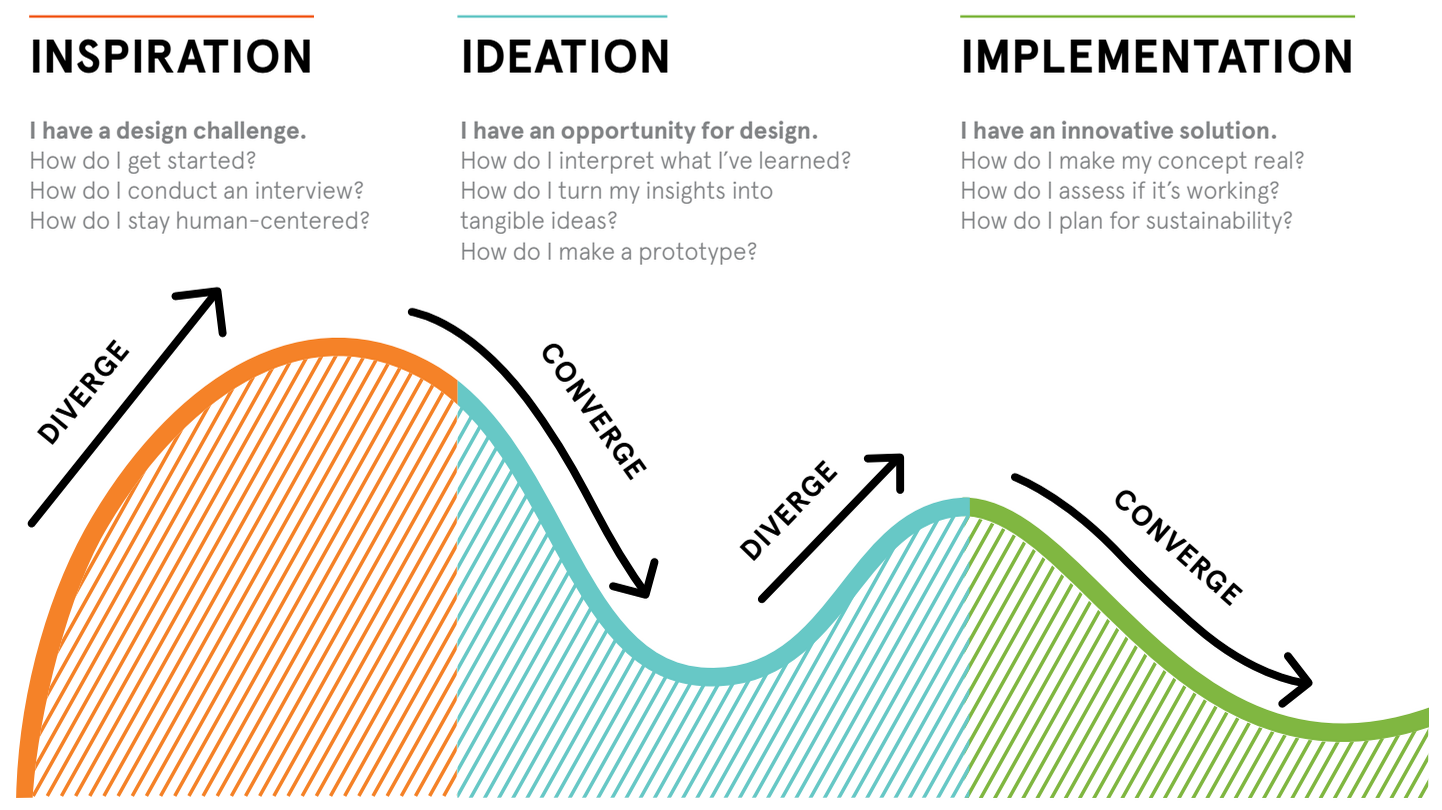
\includegraphics [width=\textwidth] {figures/IDEO.png}
    \caption{IDEO.org human-centred design process}
    \label{fig:ideo}
\end{figure}

According to \cite{Gould1985} there are three key principles of UCD: an early focus on users and tasks, empirical measurement of product usage, and iterative design. The three stages will therefore all follow the key principles of UCD, where the first stage (inspiration) will focus on user and domain research (component 1 and 2 of the personality framework), ideation will focus on designing and building the chatbot prototype and define the personality (component 3 and 4 of the personality framework), and implementation will focus on the evaluation of the final prototype, which will evaluate the personality in regards to how it's perceived and its effects on the user experience. As a UCD approach is characterised by empirical measurement, iterative design, and focus on users, each deliverable will be empirically tested through user testing techniques in iterations to inform the final prototype, while the final evaluation will be used to gather quantitative data to answer the second research question, and belonging hypotheses (stated in \ref{experimentdesign}).

\vspace{5mm} %5mm vertical space

\subsection{The Brand Mission, Goals, and Values}

To design a chatbot that conforms to the brand it represents, the brand image was analysed and defined. The mission statement was identified, the company and core values was defined, and a tone-of-voice analysis was conducted.
    
\vspace{2,5mm}
    
        \subsubsection{Mission statement and core values}
 
        The brand describes itself as having a broad social responsibility. They supply fruits and vegetables, with suppliers on all continents providing products from all over the world. Freshness is the top priority and high quality. In addition to providing fresh produce, the brand recognises having a fair and sustainable business model, which extends to proper nutrition, increased activity, and societal and environmental responsibilities. Their goal is to increase the consumption of fruit and vegetables, therefore in addition to supplying fresh produce, they take an active role in increasing knowledge and engagement regarding healthy lifestyles and positive societal development.
 
\vspace{2,5mm}
  
        \subsubsection{Mission: Fresher and healthier}
        Taken a society position in the  market that contributes to increased focus on healthy diets and physical activity. A driver and pioneer for sustainable development regarding the environment and societal responsibility within the company’s product area.
        
\vspace{2,5mm}

        \subsubsection{Brand Values}
        
        To create value for the customers, is the brand's driving force throughout the business. The conduct of employees are characterised by the values stated in the first column in Table \ref{table:1} and the core values in the second column:
        
    \begin{table}[h]
    \begin{tabular}{ |p{9cm}||p{5,4cm}|  }
     \hline
     Internal Values & Core Values \\
     \hline
        Team spirit & Vital \\
        Courage to do the right thing: Openness, honesty, probity & Current\\
        Compassion: mutual respect, care, and tolerance & Fresh \\
        & Daring    \\
     \hline
    \end{tabular}
    \caption{Internal values and core values}
    \label{table:1}
    \end{table}

    \subsubsection{Tone of Voice analysis}
    
    If the chatbot are to be perceived as an extension or continuation of the brand, it must adhere to the brands tone-of-voice. Tone-of-voice is defined as a brands personality, communicated through its written communication as well as the visual communication. Norman \& Nielsen \citep{meyer-2016} defined a framework to determine tone-of-voice based on 4 dimension: funny vs. serious, formal vs. causal, respectful vs. irreverent, enthusiastic vs. matter-of-fact.
    
    \begin{figure}
    \centering
    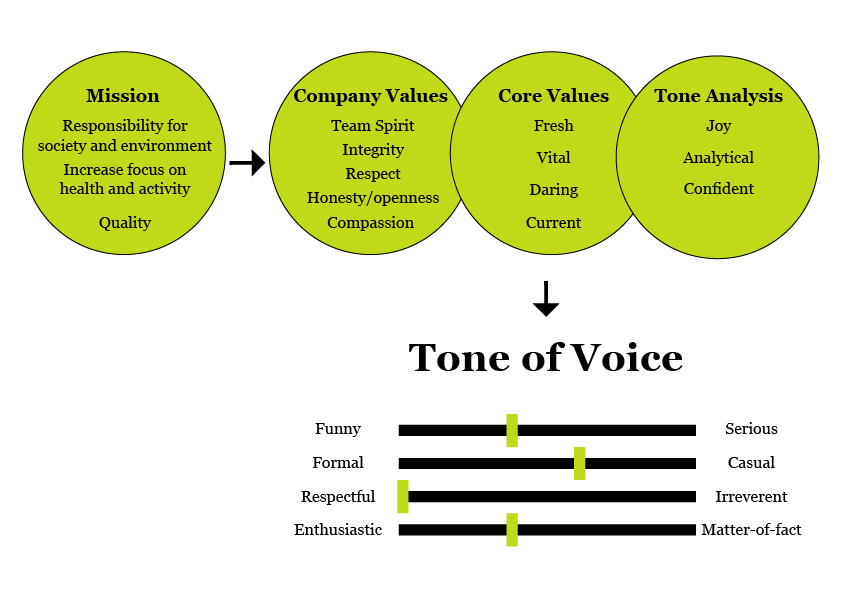
\includegraphics[width=\textwidth]{figures/Tone-of-voice.png}
    \caption{This figure shows how the tone-of-voice was defined by understanding the mission, the values and conducting a tone analysis of the written copy}
    \label{fig:tov}
    \end{figure}
    
    Figure \ref{fig:tov} shows how the tone-of-voice was determined by assessing the mission statement, the company's values inwards and outwards, and through a tone analysis. The tone analysis was conducted using the IBM tone analyser tool, the analyser assessed the written copy found on the brands website. Their tone-of-voice as reflected in their copy is more serious than funny, but not too serious as the tone is also a nice in-between of formal and casual. Their tone is very respectful, which follows their core values of tolerance and respectfulness. Lastly they are leaning towards more enthusiastic than matter-of-fact as they carry a very positive and joyful view of the future and their path to fulfil their goals.

\vspace{5mm}

\subsection{Understanding User Needs}
    
To meet the second component; to build a deep understanding of the users and their needs,  both primary and secondary research was gathered in order to understand the user group, trends, causes and statistics regarding healthy eating and food waste. 
  
\vspace{2,5mm} %2,5mm vertical space

    \subsubsection{User Interviews}
        \label{userinterview}
    A series of interviews was conducted in order to understand the experiences of the users; how do they view their intake of fruit and vegetables, what obstacles and challenges do they face, how they assess their own habits, and their thoughts regarding food waste etc. Eight users were recruited to participate in these interviews, or four couples, in the ages of 29 to 36, four mothers and four fathers. All four couples had two children in kindergarten and/or early elementary school age. Six of the participants works full time, while one mother was on maternal leave as the interviews were conducted. Two participants, one male and one female, were part-time workers and/or students at the time of the interviews. The interview guides prepared were semi-structured and aimed at mapping the daily routines, views, habits, pains and frustrations of the users during an average week. In particular the interviews aimed to see how parents assess their own eating and activity habits, and whether they are aware of food waste occurring and if so why. The interview guide can be found in Appendix \ref{interviewguide}. 
  
\vspace{2,5mm} %2,5mm vertical space

    \subsubsection{User Personas and User Scenarios}
        \label{persscen}
    Based on the findings from the user interviews and information from secondary research, two user personas were developed, one male and one female, (see \ref{Userpersona}), to summarise the user research and inform the personality of the chatbot. The user personas describes which goals the users have, as well as their frustrations and pains during an average week, what motivations that drives them and their specific needs. The user persona acts as a summary of the insights from user research, and are helpful tools to inform the requirements of the system. By understanding users' preferences, goals and pains will help determine suitable characteristics and personality traits. If the frustrations are related to feeling like you never have the time to achieve everything you wish to do in a day, a lecturing tone might not help ease this frustration, but rather increase it. The personas are therefore helpful to understand which traits that are appropriate and supports the goals of the users. The personas were used alongside other important findings to write specific user scenarios in which the chatbot solves a problem or need for the user. The user scenarios followed the method laid out by \cite{Benyon2014}, which uses insights from user research to describe user stories, to conceptual scenarios, to concrete scenarios to use cases (see figure \ref{fig:scen}). Examples of the conceptual stories can be found in \ref{Userscenarios}. The use cases formed the conversation flows, an example of these can be found in \ref{converflow}. The most important tasks that added the most value to users, was to make use of the chatbots AI to make planning dinners easier. Therefore the chatbot will help its users with planning meals on a weekly basis, each recipe will provide the necessary nutritional value needed for each member of the family, and the recipes will be "smart": generate grocery lists automatically and ensure as little leftovers as possible (both in the fridge/cupboards and on the plate). This will guarantee healthy eating for all users, decrease the needs for trips to the grocery store, and prevent food waste to a degree.
    
     \begin{figure}
            \centering
            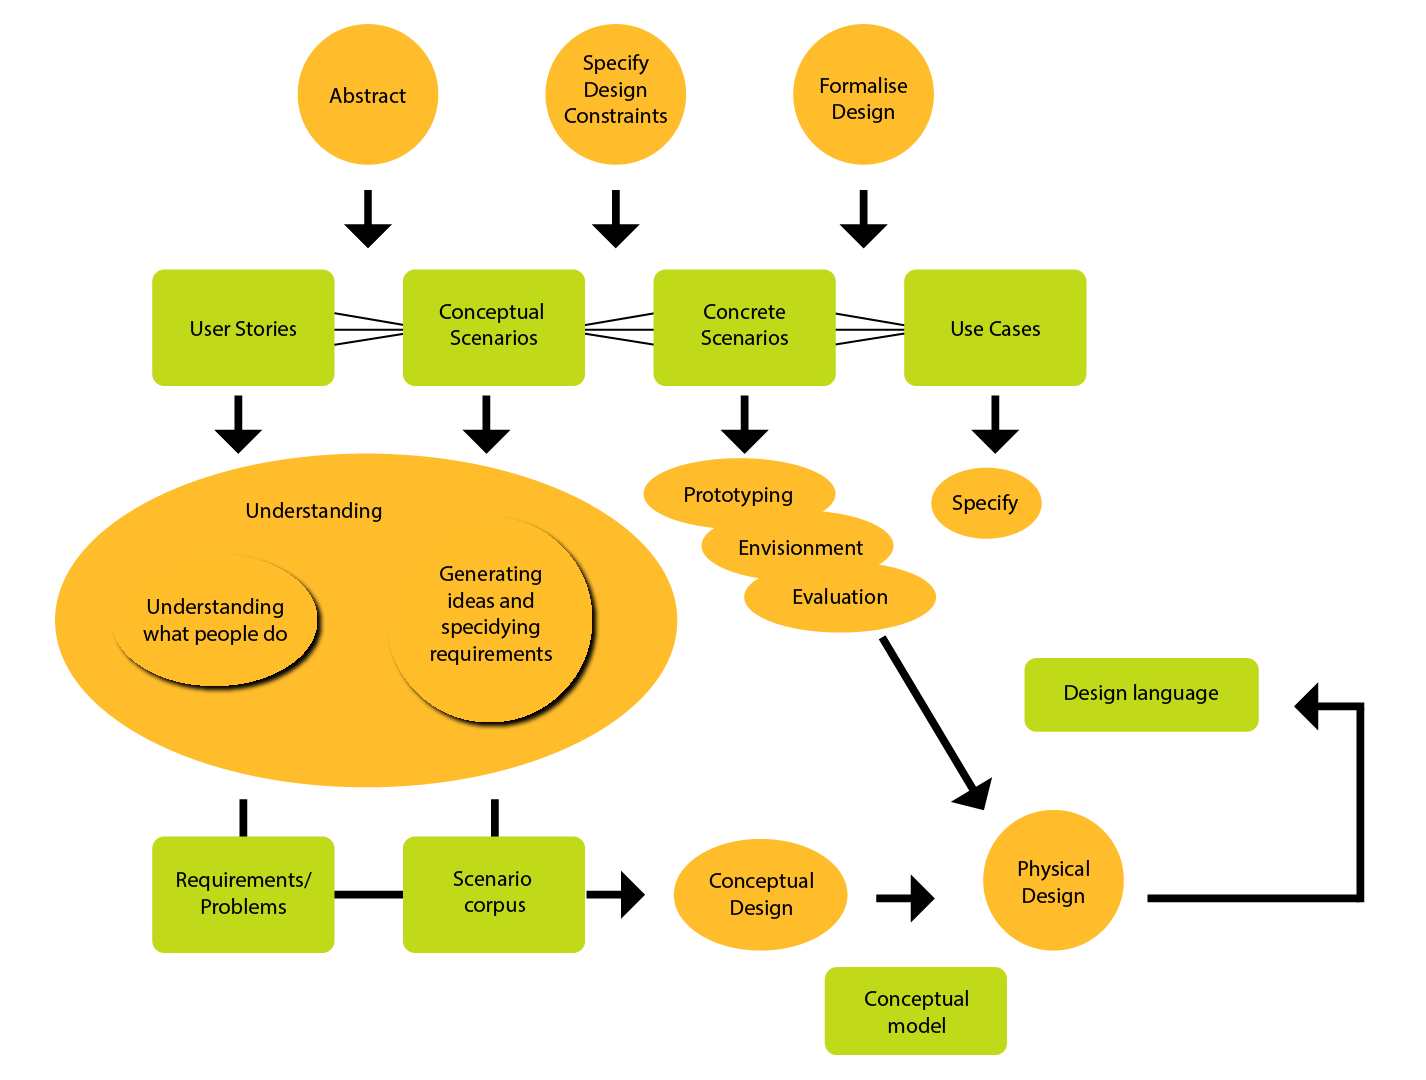
\includegraphics[width=\textwidth]{figures/Scenariobasedmethod.png}
            \caption{Scenario-based design method as discussed in \cite{Benyon2014}}
            \label{fig:scen}
        \end{figure}
    
\vspace{2,5mm} %2,5mm vertical space

    \subsection{The Chatbot Role}
    
    The third component of the personality framework consists of understanding the role the chatbot should play, or the job it should do. The user-centred approach identified the two most important jobs the chatbot could do that both furthers the goals of the brand and add value to the users: increase the consumption of fruits and vegetables, and reduce food waste. Therefore, the job of the chatbot agent is to \textit{assist} users to help them make healthier choices for their family and \textit{motivate} them to successfully implement these changes. The chatbot is there to assist and guide the users, with the long term goal of successfully implementing a fresher and healthier lifestyle and reduce food waste. 
    
    To achieve this the chatbot will help parents plan their dinners for the whole week, assist with the shopping and make recommendations based on ingredients they have in house and leftovers. In addition to this the chatbot encourages parents to inform the chatbot about what they have eaten so far, what was a success and what was not so that the chatbot can learn which items are not eaten, are wasted and instead offer healthy alternatives that will be eaten rather than wasted. 
    
    Assistants and motivators have specific traits \citep{burge2016,lipcamon_2013} in which they need to have in order to be successful in their role (see table \ref{table:2}).
    
\vspace{2,5mm}

    \begin{table}[h]
    \begin{tabular}{ |p{7,2cm}||p{7,2cm}|  }
    \hline
    Assistant & Motivator \\
    \hline
        Professionalism & Give praise and encouragement \\
        Collaborators & Treat clients as equals \\
        Outstanding organisational skills & Show trust \\
        Excellent communication skills & Communicate and set goals \\
        Willingness to go the extra miles & Be attentive \\
        Problem-solver & Allow mistakes \\
        Proactive & Be pleasant \\
        Respectful & Ask for feedback \\
        & Keep others informed \\
        & Don’t micromanage \\
    \hline
    \end{tabular}
    \caption{Desirable traits for Assistants and Motivators}
    \label{table:2}
    \end{table}
 
    The traits of the assistant will be reflected in the way the chatbot handles its job. Through AI and NLP capabilities, as well as connection to necessary APIs, will the chatbot be able to complete necessary tasks and incorporate “hidden/invisible” features that will help users achieve their goals. As for the motivator traits, this will be reflected in how it encourages/motivates users, the language its using, and its behaviour (prompts, affirmations, tips). Therefore the chatbot role will be reflected by its external traits (motivator) and its internal traits (assistant).
    
\vspace{5mm}

    \subsection{Personality Trait Model}
    Once the brand mission, core values, understanding of user needs, and the chatbot role have been identified, designers should find an appropriate personality trait model to help put together a dynamic personality for the chatbot. It is important that this model will be used to place the desired personality within a framework, this is to benefit the designer when designing a consistent personality. 
    
    It is not the goal of this thesis to assess whether the designed personality is consistent with the chosen trait model, or to assess the personality of participants. The trait model is only used to guide the design of the chatbot personality, and to help in evaluating desirable traits for the specific chatbot agent. 
    
    The chosen personality model to model this chatbot's personality was the five factor model. As explained in section 2.3.2, this personality trait model is widely known, and based on lexical data used by humans to describe personalities. These traits have been mapped out and organised into the five factors, and as the traits are identified by the words we use to describe them, it will be an appropriate model for a linguistic interface such as a chatbot.
    
\vspace{5mm}

    \subsection{The Chatbot Personality Description}
    The final chatbot personality therefore were based on identified user needs and user personas, the brand image and tone of voice, and the identified role of the chatbot. This information was used to model the desirable traits and quirks of the chatbot personality, and the five factor model was used as reference to model the personality. The personality includes the traits shown in Figure \ref{fig:characteristics}. The role and character description is laid out in next two sections; both descriptions are based on the user research in regards to how the chatbot's tone and tasks are handled to support the needs and goals of both genders.
    
    \begin{figure}[h]
            \centering
            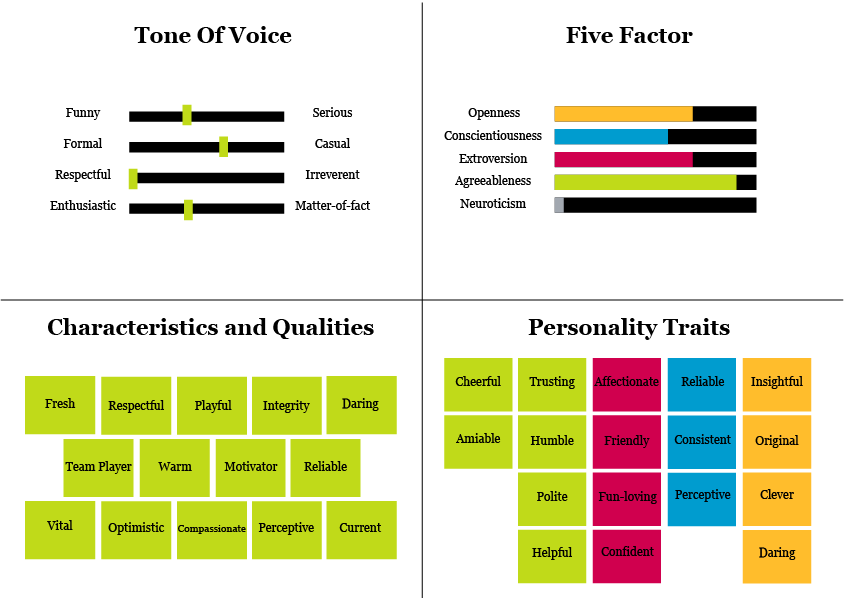
\includegraphics[scale=0.5]{figures/Defined_characteristics_and_traits.png}
            \caption{The defined tone-of-voice, five factor personality traits, characteristics and qualities}
            \label{fig:characteristics}
        \end{figure}
    
    \subsubsection{Role description}
    The chatbot has been given the name Bella. She works as a dinner planner, helping couples plan meals for the whole week. Her recipes helps couples eat a healthy and balanced diet focusing on increasing the consumption of fruits and vegetables. Bella is personalised to each specific family as she knows and learns over time what they prefer to eat, what they dislike, any known allergies they might have, and who makes up the whole family. Her mission is to increase their health, while also taking an environmental and economical approach to dinner planning; keeping track of what food they have at home, base recipes on ingredients that needs to be used up and providing users with shopping lists. It is important that Bella works to motivate users towards their goals, and does so in a supportive fashion. Her role as assistant makes sure that she is trustworthy, reliable and efficient.
    
    \subsubsection{Character description}
    Bella is designed to act and look about the same age as her target audience, she is an assistant and motivator for both genders. Her personality is modelled to be that of a supportive friend, helping with cool new tricks as well as emotional support, by using a cheerful and playful tone. Bella is designed to be used in two ways; 1) throughout the day, to log meals, ask for help and tricks, 2) when in need of reminders, accessing shopping lists and recipes on the go. Therefore Bella acts efficiently and to the point, while also providing a helpful and supportive tone. She is cheerful, youthful, and fun-loving, while also being reliant, consistent, efficient and trusting. Bella is a team player, and works to support great collaboration between couples. 

\vspace{5mm}

\section{Prototype \& Conversation Design}
The chatbot prototype was built using the Chatfuel bot builder platform, and the experiment was run through Facebook's Messenger platform. The conversation design was written by mixing a user scenario technique with mind-mapping tools, such as Xmind, to map out the different chatbot skills, user intentions, and conversation flows (see \ref{persscen} \& \ref{Userscenarios}). To improve the AI of the chatbot, the researcher wrote more than 300 unique training data per chatbot skill. This resulted in participants testing eight different conversation flows, three of which can be seen in figure \ref{fig:convflow}. These eight chatbot skills included, planning dinner for the whole week or specific day, help using leftover ingredients, log five a day, help eating healthier or increase consumption of vegetables, add and locate shopping lists.
    
\begin{figure}[H]
    \centering
    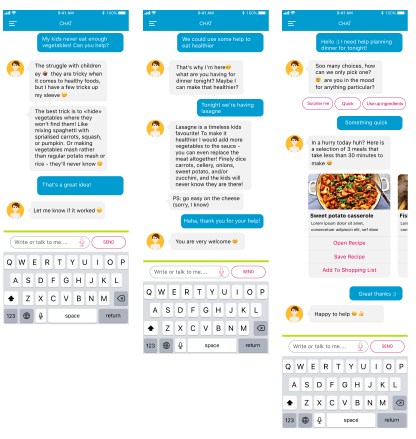
\includegraphics {figures/conversationflow_2.png}
    \caption{Example of conversations users had with Bella}
    \label{fig:convflow}
\end{figure}
    
The conversation design began by forming different use cases, that were based on the concrete scenarios built around the insights from the user interviews. These use cases described the most important tasks the chatbot could provide to its users, and the conversations were written around these tasks. The goal of the conversation would be to complete the specific task described in the use case, and this of course can be done in many different ways, which gives you the possibility to play around with multiple paths to the same conversation goal. The main path was first identified, before creating different "sub-paths" to reach the same goal. 
    
Training data for chatbots consists of variations of the user intention. This means as many versions of the same question or user input that describes the same goal. The training data is what builds the chatbots AI, and the more training data a chatbot has the more certain it becomes in predicting the right intent. If the chatbot is very well trained, it would be able to answer questions or input that has not been included in the training set, but describes the same intent.

        
\vspace{5mm}

    \subsection{The Chatbot Avatar}
    The literature review investigated how humans perceive the various types of conversational agents, and found that anthropomorphism can benefit how a personality is perceived, and that a consistent personality dictates which characteristics humans assign to a chatbot in which they anthropomorphise. The literature review also discussed humanness as it related to human capabilities and physical characteristics. The review found that chatbots with a high level of humanness increases trust and familiarity, while also providing a more natural interaction with humans. The latter is explained by that humans know how to interact with other humans, therefore will assume that a chatbot will interact like a human if it has a more human appearance. 
        
    Because of this, the chatbot avatar will have a human appearance. This chatbot is taking on human tasks and is to be perceived as a human. However, research have found that too human might have a negative effect on human perception which is why the chatbot will be portrayed as an illustrated character rather than a realistic human, as can be seen in figure \ref{fig:avatar}. This will make clear the distinction that the chatbot is not a human, while incorporating high levels of humanness simultaneously, which will contribute to increased anthropomorphism.
    
    \begin{figure}[H]
        \centering
        
\includegraphics[scale=0.35]{figures/Bella_avatar.png}
        \caption{Chatbot Bella's avatar}
        \label{fig:avatar}
    \end{figure}
    
\vspace{5mm}

\section{Chatbot B - the other chatbot}
In order to test whether the chatbot personality has any impact on the user experience, the experiment will test two levels of personality. The first level (Chatbot A) will include the personality modelled using the developed personality framework. The second level (Chatbot B), will be designed to appear as opposite to the personality of Chatbot A. This will mainly involve using the same traits that Chatbot A's personality has been modelled on and to the extent possible remove them from the personality of Chatbot B. Chatbot B will therefore appear as having a less human personality than Chatbot A. Chatbot B cannot be defined as having "no personality", as even a "machine-like" behaviour can be defined as a personality type. Instead Chatbot B has been designed to be mainly task-oriented, providing the same service and completing the same task as Chatbot A, but in a machine-like way as shown in table \ref{table:3}.
    
\begin{table}[h]
\begin{tabular}{ |p{3cm}||p{5cm}||p{5cm}| }
    \hline
    User Expressions & Chatbot A & Chatbot B \\ 
    \hline
    What should I cook for dinner tonight? &    Cool cool;) What are you in the mood for?   & Do you have a preference? \\
    \hline   
    Something that's quick to make &   In a hurry today huh? Here's a selection of 3 meals that take less than 30 minutes to make  & Quick recipes: \\
    \hline
    Dinner tonight was delicious! & That's wonderful :D should I recommend this recipe again?  & OK, recommend recipe in future? \\
    \hline
\end{tabular}
\caption{Difference in personality in responses between Chatbot A and Chatbot B}
\label{table:3}
\end{table}
    
This means that Chatbot B will provide the same value to users as Chatbot A, by meeting their needs and being a great assistant. However, the motivator role will be affected by the different personalities, as Chatbot B will not act as a great motivator as these traits are mainly found in the Agreeable and Extroversion factors. Therefore Chatbot A and B will have the following traits in common: Reliable, Consistent, and Perceptive. These are the traits found in the conscientiousness factor, and mainly displayed through the assistant role. The traits found in the Openness factor will also be removed to some extent in Chatbot B, however some of the traits might be reflected in the tasks it performs and will therefore to some extent be present in Chatbot B. The prototype for Chatbot B was built by duplicating Chatbot A, and change the way it responded to fit with its defined personality characteristics.

\vspace{5mm} %5mm vertical space
    
\section{Experiment Design}
    \label{experimentdesign}

The experiment will be conducted in two parts in order to answer the second research question: \textit{Will chatbots with a defined personality improve the user experience of chatbot interfaces?}. The first part of the experiment (Experiment Part 1) consists of evaluating whether participants perceive the intended personalities for both chatbot versions. This it to control that the personality has been modelled correctly, and are perceived as such. This will also test whether the personalities are perceived consistently by all participants, and that they are in agreement. Then, the second part of the experiment (Experiment Part 2) will assess whether personality has an effect on the user experience. Each part of the experiment will be conducted simultaneously, and repeated for each chatbot version as seen in table \ref{table:expdes}.

\vspace{2,5mm}

  \begin{table}[h]
  \centering
    \begin{tabular}{ |p{1,5cm}||p{1,8cm}||p{4cm}||p{1,8cm}||p{4cm}| }
    \hline
    \multicolumn{5}{|c|}{Experiment Design} \\
    \hline
    Group 1 &   Chatbot A & Evaluation Part 1 + Evaluation Part 2 & Chatbot B & Evaluation Part 1 + Evaluation Part 2 \\
    \hline   
    Group 2 &   Chatbot B & Evaluation Part 1 + Evaluation Part 2 & Chatbot A & Evaluation Part 1 + Evaluation Part 2 \\
    \hline
    \end{tabular}
    \caption{Experiment Design showing the starting condition and when participants will evaluate the chatbot versions}
    \label{table:expdes}
    \end{table}
    
\vspace{2,5mm}

\subsection{Experiment Part 1}

\vspace{2,5mm}

\begin{tabular}{ l l }
    \textbf{Independent Variable:} & Characteristics \\ 
    \textbf{Dependent Variable:} & Personality \\  
\end{tabular}

\vspace{2,5mm}

Part 1 of the experiment, to assess whether participants perceive the intended personality, will be assessed by asking participants, after interacting with the chatbot, to rate on a five point Likert scale whether they perceived each characteristic. As seen in table \ref{table:expdes}, participants will begin with either Chatbot A or Chatbot B, asked to rate the characteristics right after the first interaction, then interact with the second chatbot and then rate the characteristics for that chatbot as well. The first part of the evaluation will use the following hypotheses:\\
    
    $H_1 1$: \textit{Users will perceive the personality of Chatbot A as different to the personality of Chatbot B}
    
    $H_0 1$: \textit{Users will not perceive the personality of Chatbot A as different to the personality of Chatbot B} \\
  
    $H_1 2$: \textit{Users will perceive the personality of Chatbot A as intended} 
    
    $H_0 2$: \textit{Users will not perceive the personality of Chatbot A as intended}\\
   
    $H_1 3$: \textit{Users will perceive the personality of Chatbot B as intended}
   
    $H_0 3$: \textit{Users will not perceive the personality of Chatbot B as intended}\\
    

\subsubsection{Data Collection Experiment Part 1}

To collect the necessary data to assess the stated hypotheses for part one of the experiment, the participants will be asked to evaluate the predefined characteristics of the personalities each chatbot is modelled on, on a five-point Likert scale. The data collection forms are the same for each chatbot. The characteristics included in the data collection form are the characteristics Chatbot A's personality is modelled on, as seen in Table \ref{tab:datacolchar}. Chatbot B only has three characteristics in common with Chatbot A: 1) Reliable 2) consistent 3) Perceptive, which are found in the conscientiousness factor. Therefore, if the personality for Chatbot A and the personality for Chatbot B is perceived as intended, the results should have these three characteristics rated to a high degree by all participants. All other characteristics should be rated to a low degree for Chatbot B, and to a high degree for Chatbot A. This experiment is conducted to determine to what extent participants perceived the given traits, and whether participants are in agreement of the perceived traits. This will help determine whether the chatbot script has been successful in displaying the correct and intended personality; or whether participants perceive a different personality for one or both chatbot versions. It will also inform to what degree the two personalities are seen as different by all participants. All participants will be subject to all conditions, and asked to evaluate each chatbot versions independently. 

\vspace{2,5mm}

\begin{table}[H]
    \centering
\begin{tabular}{|p{2cm}|p{2cm}|p{2cm}|p{2cm}|p{2cm}|p{2cm}|}
 \hline
 \multicolumn{6}{|c|}{Characteristics Data Collection Form} \\
 \hline
& 1=not at all & 2=to a small degree & 3=to some extent & 4=to a high degree & 5=to a very high degree \\
\hline
Cheerful & & & & & \\
\hline
Trusting & & & & & \\
\hline
Polite & & & & & \\
\hline
Helpful & & & & & \\
\hline
Affectionate & & & & & \\
\hline
Reliable & & & & & \\
\hline
Fun-loving & & & & & \\
\hline
Confident & & & & & \\
\hline
Consistent & & & & & \\
\hline
Perceptive & & & & & \\
\hline
Insightful & & & & & \\
\hline
Original & & & & & \\
\hline
Clever & & & & & \\
\hline
Daring & & & & & \\
\hline
\end{tabular}
 \caption{Data collection form presented to each participant to rate the chatbot personality against the given characteristics}
    \label{tab:datacolchar}
\end{table}


\subsection{Experiment Part 2}

\vspace{2,5mm}

\begin{tabular}[h]{ l l }
    \textbf{Independent Variable:} & Personality \\ 
    \textbf{Dependent Variable:} & User Experience \\  
\end{tabular}
    
\vspace{2,5mm}

Part two of the experiment will be conducted to assess whether personality affects the user experience, and will do this by manipulating the independent variable \textit{Personality} into two levels (Chatbot A and B), to assess whether it has an effect on the dependent variable \textit{User Experience}. The second part of the experiment uses the following hypotheses:\\
    
    
    $H_1 4$: \textit{Personality affects the user experience of chatbots}
    
    $H_0 4$: \textit{Personality has no effect on the user experience of chatbots} \\
    
    $H_1 5$: \textit{Chatbot A will have an improved effect over Chatbot B} 
    
    $H_0 5$: \textit{Chatbot A will not have an improved effect over Chatbot B} \\
    
    In addition to these hypotheses the researcher will also collect data on each participants preferred version as well as their reasoning for this. The researcher assumes that the motivator role might be more appropriate for female users, especially if they are mothers, as they are more likely to use the chatbot throughout the day for help and guidance, while male users are more concerned with how efficiently and usable it is in completing tasks. Therefore collecting additional data on preference and reasoning, might help inform this assumption and could be interesting to see next to the final results.
    
    \vspace{5mm} %5mm vertical space
    
\subsubsection{Data Collection Experiment Part 2}
To collect the necessary data to assess the stated hypotheses for the second part of the experiment, the AttrakDiff measuring tool will be used to assess the effect on the user experience. All participants will be subject to all conditions, and asked to evaluate each chatbot versions independently.

    \vspace{5mm} %5mm vertical space
   
    \subsubsection{AttrakDiff - operationalising the user experience}
    
    User experience is defined in ISO 9241 – 210 as "all the users' emotions beliefs, preferences, perceptions, physical and psychological responses, behaviours, and accomplishments that occur before, during and after use" \citep{ISO9241-210}. Usability is the most widely known definition to determine whether a product is good or bad, and therefore an important part to determine a great user experience. Usability is defined in ISO 9241-210 as the "extent to which a system, product or service can be used by specified users to achieve specified goals with effectiveness, efficiency and satisfaction in a specified context of use". Hassenzahl (2006) believes that this definition is too task oriented, focusing on task completion and reaching goals, simplicity and efficiency, and forgetting about the "fun". Satisfaction is therefore one of the components of usability in which professionals, researchers, and designers alike struggle to agree on a definition. Is it the satisfaction of efficiently completing a task, or the satisfaction of an overall enjoyable experience? The AttrakDiff measurement tool was built to assess exactly this, knowing that users might choose a product which is slightly less efficient but are extremely enjoyable to use. While some argue that something cannot be enjoyable unless it is efficient, we must not forget all the different ways in which the overall user experience is affected by a product that "stands out" from the rest. \cite{Hassenzahl2000} built the AttrakDiff measurement tool, which assesses the user experience by looking at usefulness and usability in the pragmatic quality, independently from the hedonic qualities of stimulation, challenge and motivation, and attractiveness. The AttrakDiff form assesses personal user rating of a products usability and design.
    
     \begin{itemize}
        \item Pragmatic Quality: Usefulness and usability of the system
        \item Hedonic Quality: Motivation, stimulation and challenge for the user
    \end{itemize}
    
    The AttrakDiff measurement instrument consists of 28 seven-step items of opposite adjectives ordered into a scale of intensity \citep{attrakdiff2013}. The middle values of an item group creates a scale value for pragmatic quality (PQ), hedonic quality (HQ - include HQ-I and HQ-S) and attractiveness (ATT). HQ-I and HQ-S are the sub-qualities of stimulation and identity of hedonic quality. The theoretical model was created and tested by Hassenzahl et al. from 2000 through 2006 \citep{Hassenzahl2000, Hassenzahl2001}; and their studies have found that the hedonic and pragmatic qualities are perceived independently from each other and consistently, and contributes equally to the attractiveness rating. According to their website, Hassenzhal et al. (2000) found that the model separates four essential aspects: 1) the product quality intended by the designer, 2) the subjective perception and evaluation of quality, 3) the independent pragmatic and hedonic qualities, and 4) the behavioural and emotional consequences \citep{attrakdiff2013}.
    
    The AttrakDiff measurement tool was used to collect the appropriate data to assess and compare the two chatbot personalities against the user experience. The AttrakDiff evaluation will be used to assess the user experience of both chatbot prototypes. The pragmatic quality will asses usability and usefulness of the chatbot, while both hedonic and attractiveness qualities will be used to assess the satisfaction with each version.
    
    \subsection{Experiment Setup}
    
    Participants were recruited through convenience sampling, all participants were within the age group of 25-40 years of age, the sample consisted of couples, either married or unmarried, but all living together. 12 of the 16 participants had children in kindergarten or elementary school, while two couples are not parents as of yet. Eight of the participants had also participated in the earlier interviews. The participants were invited to test a new chatbot application that aims to help families with weekly tasks. This means that none of the participants were aware that the goal of the experiment is to test the chatbot personality, but rather that they were invited to test two versions of a chatbot interface. Before the participants began the tests, they were given one deck of eight cards, see figure \ref{fig:userneed}, each describing a need participants have. Participants will be asked to open one card at a time and use the chatbot to solve that need e.g. "I don't know what I should make for dinner tonight". In addition to this deck participants will also be presented with four different coloured decks, see figure \ref{fig:dinnerveg} and \ref{fig:ingfruit}, they will be asked to open one card from each of the four decks that are named: 1) Dinner 2) Ingredient 3) Vegetables 4) Fruits. Participants were instructed to provide this information when asked by the chatbot. E.g. one of the conversation flows includes adding an ingredient to the shopping list, your ingredient card informs the participant which ingredient to add. The cards were necessary as it was important that the experiment was completed with as little interference from the test moderator as possible. This was to not influence ones own personality into the interaction with the chatbot solution. The two chatbot versions are prototypes, and therefore prone to error during testing. Time restraints made it impossible to produce a complete well-functioning chatbot, this made it necessary to design the experiment to only include specific conversation flows presented by the cards mentioned above. Pilot studies and preliminary studies conducted during the autumn 2017, found that errors occurring during a chatbot user test has a huge impact on participant's perception of the chatbot as a whole, as participants rated the chatbot as being lower in intelligence, helpfulness, and usefulness if it predicted the wrong intent. Therefore it is very important that the chatbot does not give a wrong answer or fail to predict the right answer during the experiment. 
   
    \begin{figure}[h]
            \centering
            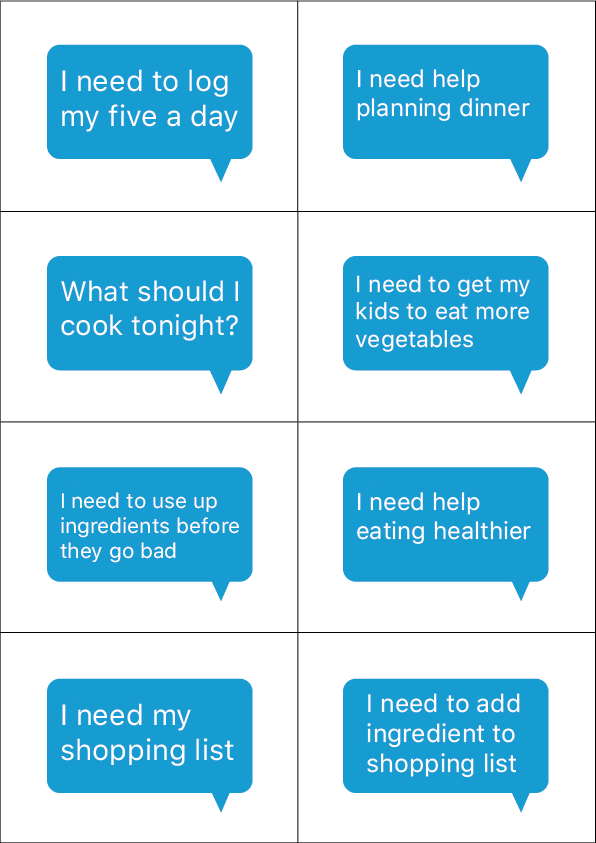
\includegraphics[scale=0.5]{figures/userneeds.png}
            \caption{Figure showing the eight cards with a need to be solved by the chatbot}
            \label{fig:userneed}
        \end{figure}
        
    \begin{figure}[h]
            \centering
            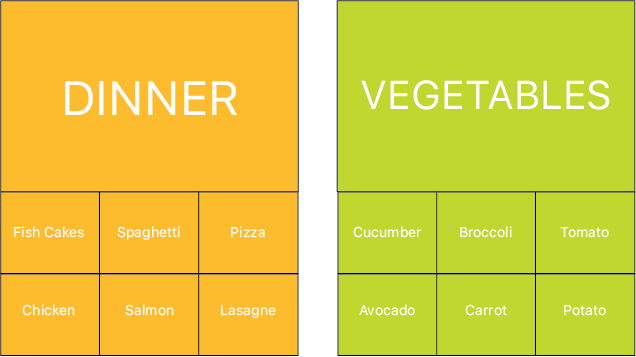
\includegraphics[scale=0.5]{figures/dinnerveg.png}
            \caption{Figure showing the cards for dinners and vegetables}
            \label{fig:dinnerveg}
        \end{figure}
        
     \begin{figure}[h]
            \centering
            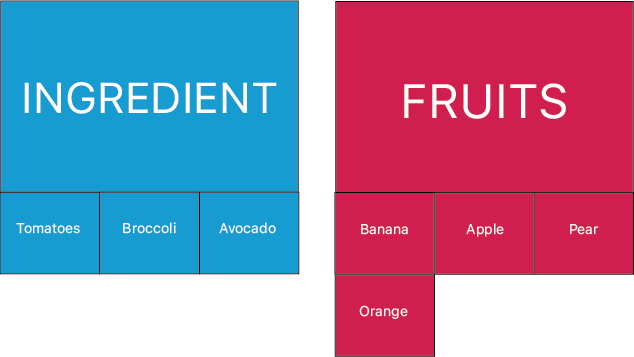
\includegraphics[scale=0.5]{figures/Ingredientfruit.png}
            \caption{Figure showing the cards for ingredients and fruits}
            \label{fig:ingfruit}
        \end{figure}

   The decks were necessary to exclude any interference from the researcher, and also ensured that participants were engaged in conversations flows that the chatbot had been trained to know well. This allowed the researcher to focus on only eight specific conversations to allow participants to interact with the system. The preliminary study conducted as preparation for this master project found that users need a goal with the interaction and expect a chatbot to be able to do something, or perform some kind of service, to perceive the interaction as meaningful. Participants were unable to give a true evaluation of their perception in the preliminary study if they did not "see the point" with the interaction, as there was a conflict when rating characteristics such as intelligent or helpful. Therefore, participants will use the chatbot as a complete service, even though the research aim is not to assess how well the chatbot performs its tasks. In order to conduct a true assessment of user experience, the product being tested must be seen as useful to its users, this will be reflected in the pragmatic quality score from the AttrakDiff test. The design process and participant sampling will already have assured that the tasks the chatbot performs are valuable or useful to the participants, which means that the Pragmatic Quality of each version is assumed to be scored high by all participants - although maybe not to the same degree.
   
   \begin{table}[h]
    \begin{tabular}{ |p{3cm}||p{5cm}||p{5cm}| }
    \hline
    \multicolumn{3}{|c|}{Experiment Design} \\
    \hline
    Group 1 &   Chatbot A & Chatbot B \\
    \hline   
    Group 2 &   Chatbot B & Chatbot A \\
    \hline
    \end{tabular}
    \caption{Within-subjects design to control for confounding variables}
    \label{table:4}
    \end{table}
   
   Participants will evaluate the two chatbots by completing a series of tasks using each chatbot. As mentioned earlier in this chapter, the first part of the experiment will be used to assess whether the personality is perceived consistently and as intended by each participant, and the second part to assess the user experience. In order to compare the two chatbot versions, the participants will be their own control group as the experiment design will allow for a between \& within-subjects design using a two by two factorial design, see table \ref{table:4}. Half of the group will test Chatbot A first, while the second half will test Chatbot B first. This is to avoid a sequence/interaction effect, where participants become affected by which chatbot they try first. Participants will not have any comparison during the first interaction, and can therefore be either stricter or nicer in their assessment. While the second interaction will be compared to the first interaction, and can therefore also be assessed stricter or nicer. Participant's might also feel more at ease during the second interaction, as they now know what to do. After the participants have interacted with each chatbot they will be asked to assess the chatbot personality characteristics to determine whether participants are in agreement regarding the perceived characteristics and personality traits. Then participants will be asked to fill out the AttrakDiff evaluation to assess the perceived hedonic-, and pragmatic quality and attractiveness of the chatbot, before repeating the same process again with the second chatbot version. This experiment design will ensure statistic power. Both the personality characteristics data collection form and the AttrakDiff measurement tool will be presented to all participants after they have interacted with each chatbot. The participants will be presented with the same form for each bot, and the forms will be accessed locally through the researchers private computer in order to ensure participants anonymity. 
  
    
